% NS-022 assembled manuscript: reviewed non-result fragments plus actual
% 32-cell A/B local-cold results. Official style remains anonymous default.
% Classic xref (no object streams) keeps the compiled PDF UTF-8 text so the
% declared paper.pdf and its receipt snapshot are not an unlisted binary.
\pdfobjcompresslevel=0
\documentclass{article}
\PassOptionsToPackage{numbers,compress}{natbib}
\usepackage{neurips_2026_vericode}
\usepackage[utf8]{inputenc}
\usepackage[T1]{fontenc}
\usepackage{amsmath,amssymb,booktabs,microtype,url,graphicx,tikz,xcolor,float,hyperref}
\title{Neurosymbolic Supervision with Explicit Evidence: A Cold Repair Study}
\workshoptitle{AI for Verifiable Coding}
\author{Anonymous Authors}
\hypersetup{pdftitle={Neurosymbolic Supervision with Explicit Evidence: A Cold Repair Study},
  pdfauthor={Anonymous Authors}}
\begin{document}
\maketitle
\begin{abstract}
Coding supervisors must separate source-linked obligations from operational
decisions and from the evidence that may admit a candidate. We report a frozen
eight-family comparison of that bounded composition: whether adding native
source-linked semantic context to matched public raw context changes useful
cold repair under a fixed resource policy. The retained design is 32~fixed
A/B local-cold cells across eight convenience-selected repository families
and two nested repetitions ($104729$, $130363$), an order-preserving subset of
an original 192-cell plan. Useful completion is $9/32$ (arm~A $5/16$, arm~B
$4/16$). The mean family B-minus-A useful fraction is $-0.0625$, with a
descriptive conditional 95\% percentile interval $[-0.1875,0]$ from $20{,}000$
whole-family bootstrap resamples. Sixteen scoring invocations produced
fifteen completed cold validations; one additional scored cell had incomplete
hidden collection. Fourteen cells hit child deadlines and two were known
proposal failures. All 32~cells remain in the denominator. C/D routing, warm
caches, reuse, publication-comparison efficacy, and original sixteen-family
inferential objectives were withdrawn before outcomes. Human semantic fidelity
was not measured. Settled provider charges remain unavailable. The result is
descriptive of these eight families; it does not establish superiority,
noninferiority, or population-level coverage.
\end{abstract}

\section{Introduction}
\label{sec:introduction}

A coding supervisor must distinguish what an edit changes, what evidence
applies to the resulting program, and who may accept the transition. A stored
passing result can concern an earlier source revision; a completed task can
record an operational decision without establishing a behavioral property.
Repository-agent interfaces and test-validation benchmarks make the boundary
between proposals and checks central to useful repair~\citep{baseline08,baseline11}.
Our starting point is to make each observation's subject, scope, and authority
explicit.

The architecture separates semantic state, which records source-linked facts
and unresolved obligations, from operational state, which records work and
decisions, and artifact storage, which retains candidate bytes and evidence.
A proposed transition identifies evidence for its declared acceptance
conditions. Unknown dependencies and unsupported translations remain visible
obligations. Neither persistence nor a cryptographic commitment turns an
observation into proof of an unstated property.

The contribution is a design for these evidence boundaries, conditional
acceptance and reuse arguments, and a bounded implementation comparison.
The empirical question is whether adding native source-linked semantic
context to matched public raw context changes useful cold repair under a
fixed resource policy. The retained design contains eight repository families,
two arms, and two nested repetitions per arm. It tests the combined context
mechanism, rather than every component of the intended supervision loop.
Symbolic routing, warm-cache reuse, publication efficacy, and native proving
performance require separate evidence.

A returned proposal is not a successful repair. Useful completion requires
actual nonempty public and hidden checks to pass within the measured resource
rules; provider failures, timeouts, and incomplete validation stay in the fixed
denominator. This separation also governs the reporting of setup work, earlier
pilot results, runtime interruptions, and unknown costs.

\section{Method and trusted assumptions}
\label{sec:evidence-method}

\paragraph{Separate evidence classes.}
Semantic state links facts, dependencies, contracts, and unresolved obligations
to source. Operational state records goals, tasks, attempts, leases, and
decisions. Artifact storage preserves candidate bytes and accepted manifests.
An evidence item binds a subject to a declared statement, checker, environment,
and provenance. A passing test concerns the finite checks actually executed;
a formal derivation concerns its encoded relation and premises; a grant concerns
an actor's permission to act now. These classes cannot substitute for one another.
In particular, a signature binds a record to a key under cryptographic
assumptions. It establishes neither checker adequacy nor the honesty of an
observation.

\paragraph{Applicable evidence.}
The intended loop derives obligations from current source, chooses an
admissible analysis or proposal route, checks an isolated candidate, and admits
only evidence applicable to that candidate. Translation validation motivates
checking a particular conversion against its stated relation~\citep{baseline04};
a source-linked record alone is not such validation. Abstract facts likewise
depend on an approximation relation~\citep{baseline02}. A typed or
content-addressed representation does not imply full source-language soundness.

\paragraph{Conditional acceptance and reuse.}
If publication succeeds only after checking the current parent, authorized
scope, complete requirement manifest, admitted evidence, and expected-parent
compare-and-swap, each successful successor satisfies those gates. Given a valid
initial root and exclusive use of that publication operation, induction
preserves the declared manifest policy. This does not establish enforcement by
unexamined write paths or atomicity of external effects.

For test reuse, suppose the observation of test $t$ under profile $\theta$
factors through a complete dependency projection:
\[
  \operatorname{Obs}_{\theta}(t,s)=f_{\theta}(\pi_D(s)).
\]
If $f_\theta$ is deterministic on every admitted state, equal projections imply
equal observations. Completeness and determinism are substantive premises;
hashing an incomplete dependency list, opaque fixture, or uncontrolled effect
does not discharge them. Appendix~\ref{sec:formal-arguments-ns023} preserves
the full conditional, unmachine-checked statements and the distinction between
behavioral acceptance, action permission, and publication.

\paragraph{Executed scope.}
The final comparison exercises native context preparation, model proposals,
candidate custody and AI inspection, and separate cold scoring. Earlier
constructed controls and a local guard-before-write witness test named
implementation boundaries; they do not establish that the complete intended
loop ran as a live benchmark. The retained proof profile lacks the admitted
backend, key provenance, and exact statement binding required for native proof
admission. Neither native proving performance nor empirical reuse benefit is
inferred from these arguments.

\section{Frozen comparison}
\label{sec:design}

\paragraph{Population and treatment.}
The eight recruited families are Tomlkit, installer, Tornado, more-itertools,
charset-normalizer, iniconfig, wheel, and Jinja. They are a convenience sample,
not a representative sample of Python repositories. Two arms and two nested
repetitions yield 32 fixed cells, 16 per arm. Repetition identifiers 104729 and
130363 identify design positions; they were not served to the model API as
random seeds.

Before final outcomes, the A/B local-cold comparison was retained as an
order-preserving subset of the original 192-cell plan. The remaining 160 factor
cells were withdrawn, and eight additional target families were not recruited.
C/D routing, warm caches, test reuse, publication efficacy, the original
sixteen-family inferential objectives, and D/A promotion comparisons remain
outside this experiment. The narrowed comparison is descriptive.

Arm A receives the selected public raw context. Arm B preserves the matched
raw selection and adds actual native source-linked semantic context.
Sixteen exact family/arm request commitments precede final generation; each
arm's two repetitions use its fixed request. This treatment changes the
combined request and cannot isolate semantic subcomponents or prompt
compression. Public source and native preparation remain separate from
confidential acceptance tests.

\paragraph{One proposal and independent cold execution.}
Each cell permits one Grok 4.6 proposal POST, requesting at most 4,096 output
tokens through a strict structured edit response. There is no scientific
fallback, retry, served seed, or reasoning-effort parameter. A failed request
consumes its original cell rather than creating a replacement. The frozen
order is executed sequentially.

Proposal execution uses one CPU, 2~GiB, and a 32-process limit. The nominal
gateway and HTTP-wrapper bounds are 600 seconds; the child bound is 595 seconds
and the socket timeout is 590 seconds. Compliance depends on actual measured
intervals. A configured limit, missing measurement, or nonfinite value is not
evidence that the budget was met.

The operator retains exact candidate bytes and a specific AI review before
eligible scoring. That procedural review supplies no independent human
annotation. Scoring runs separately in a cold, network-disabled container with
one CPU, 2~GiB, and a 128-process limit, bounded by 120 host seconds and 115
child seconds. The scorer's process limit was fixed prospectively for both
arms and all eight families because unchanged public concurrency tests require
up to 100 threads. The earlier 32-process public-baseline failure remains
recorded; proposal and native-preparation limits remain 32.

Useful completion requires an admitted candidate, nonempty public and hidden
checks all passing, and measured resource compliance. Failed, refused,
expired, unscored, or incomplete cells receive no useful-completion credit.
Unknown states remain explicit and prevent a complete-cohort analysis until
their terminal accounting is resolved. An import or collection error with
no hidden assertions executed is incomplete validation, not an observed
hidden behavioral assertion failure. Separate scoring and sealed records do
not establish comprehensive resistance to adversarial scorer manipulation.

\paragraph{Interruption and provenance.}
The original resource lease ended during cell~7. Its request, failure, cleanup,
and unknown termination-sender evidence remain retained. A separately admitted
managed lease and continuation runtime govern cells~8--32 without replaying
the consumed prefix or changing requests, model, order, scorer, limits, or
analysis. Both runtime source versions remain explicit. The lease is a
cooperative allocation, not an exclusive physical resource reservation;
per-phase process boundaries apply the configured resource limits.

Continuation checks add work around effect admission and receipt signing.
The signed gateway interval ends before signing; whole operator invocation
time extends through subprocess completion and output flush/synchronization.
These distinct intervals must retain their endpoints rather than being
presented as a single total host clock.

\section{Analysis and evidence separation}
\label{sec:analysis-method}

For family $f$, arm $a$, and repetition $r$, let $Y_{far}$ indicate admitted
useful completion. Average the two fixed repetitions within each family and arm:
$\bar Y_{fa}=(Y_{fa1}+Y_{fa2})/2$. The retained contrast is
\[
  \widehat{\Delta}=\frac{1}{8}\sum_{f=1}^{8}
                   \bigl(\bar Y_{fB}-\bar Y_{fA}\bigr).
\]
Families are the independent analysis units; 32 nested cells are not 32
independent repositories. A descriptive robust-family outcome additionally
requires both repetitions to succeed and is not a promotion decision.

The frozen bootstrap draws eight whole family blocks with replacement, sharing
each draw across arms and repetitions. It uses 20,000 resamples, Python 3.12
\texttt{random.Random} with seed 20260911, lexicographically ordered family
identifiers, and exactly eight \texttt{randrange(8)} draws per resample.
The 95\% percentile endpoints use linear interpolation at $(B-1)p$ for
$p\in\{0.025,0.975\}$ and $B=20{,}000$. These intervals are conditional,
descriptive summaries of eight convenience-selected families, not
population-level coverage or superiority/noninferiority decisions.

Failures remain in the fixed outcome denominator. Resource summaries report
their available-observation counts and missingness. Provider child, HTTP
wrapper, gateway, scorer, and operator clocks can overlap and are not added
as disjoint costs. Shared native preparation is counted once. Baseline checks,
prior failed attempts, review, queue waits, cleanup, and artifact work retain
their own accounting scopes. Token usage and cost ticks are telemetry;
unavailable settled charges and unmeasured effort remain unknown.

The developmental pilot is a separate four-family, 24-cell A/B study with
three nested repetitions. Its retained labels include ten useful completions,
five per arm, from 24 POSTs and 12 scores. Ten child durations exceeded 595
seconds by less than 1~ms, and pilot cell~20 exceeded 600 seconds in both
wrapper and gateway clocks. These deviations and labels remain preserved;
the final resource policy is not applied retrospectively to relabel the pilot.

Earlier boundary evidence is also separate from final repair outcomes.
The mutation/cold comparison retains one false reuse among all 26 cases,
rather than reporting a selected zero-of-25 subset. All four later correction
invocations, including failed and partial attempts, remain visible; corrected
full-cold execution supplies no positive reuse credit. Constructed gate checks
and public-baseline passes do not count as useful final repairs.

\section{Results}
\label{sec:results}

All 32 planned cells are terminal. Useful completion is $9/32$
($0.28125$): arm~A $5/16$ and arm~B $4/16$. Mean family B-minus-A useful
fraction is $-0.0625$. The frozen $20{,}000$-resample whole-family percentile
interval is $[-0.1875,0]$ and is not degenerate. The interval includes $0$ and
does not support a superiority, noninferiority, equality, or safety claim.
Table~\ref{tab:family-useful} and Figure~\ref{fig:family-useful} report the
eight family blocks. Tornado is the only family whose two-repetition means
differ (A both useful; B one useful). Tomlkit and more-itertools are tied;
the other five families contribute zeros on both arms.

\begin{table}[H]
  \caption{Useful completions among two nested repetitions per family and arm.
    Families are the analysis blocks. Generated from the complete 32-cell
    analysis; repetitions are nested, not independent repositories.}
  \label{tab:family-useful}
  \centering
  \begin{tabular}{lrrr}
\hline
Family & A useful / 2 & B useful / 2 & B$-$A mean \\
\hline
09-tomlkit & 1 & 1 & 0 \\
10-installer & 0 & 0 & 0 \\
11-tornado & 2 & 1 & -0.5 \\
12-more-itertools & 2 & 2 & 0 \\
13-charset\_normalizer & 0 & 0 & 0 \\
14-iniconfig & 0 & 0 & 0 \\
15-wheel & 0 & 0 & 0 \\
16-jinja & 0 & 0 & 0 \\
\hline
All eight (16 cells per arm) & 5 / 16 & 4 / 16 & -0.0625 \\
\hline
\end{tabular}
% Repetitions are nested; the eight families are the analysis blocks.

\end{table}

\begin{figure}[H]
  \centering
  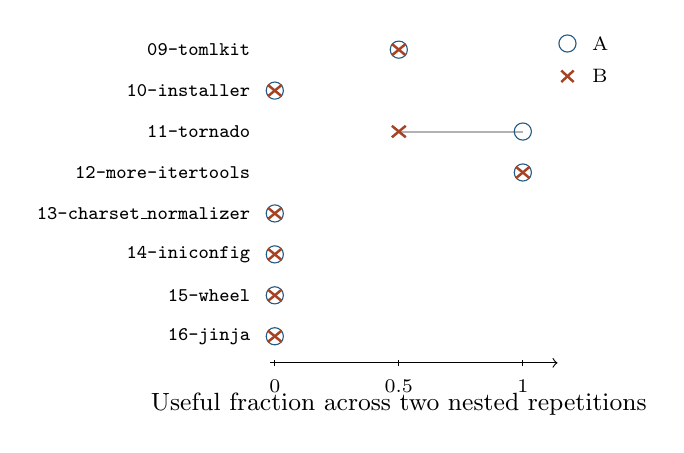
\begin{tikzpicture}[x=3.15cm,y=0.52cm]
    \definecolor{armA}{HTML}{245A81}
    \definecolor{armB}{HTML}{A64324}
    \foreach \y/\name/\a/\b in {
      8/09-tomlkit/0.5/0.5,
      7/10-installer/0.0/0.0,
      6/11-tornado/1.0/0.5,
      5/12-more-itertools/1.0/1.0,
      4/13-charset\_normalizer/0.0/0.0,
      3/14-iniconfig/0.0/0.0,
      2/15-wheel/0.0/0.0,
      1/16-jinja/0.0/0.0} {
      \node[font=\scriptsize,anchor=east] at (-0.06,\y) {\texttt{\name}};
      \draw[color=black!30,line width=0.7pt] (\a,\y) -- (\b,\y);
      \draw[armA,thin] (\a,\y) circle (3.1pt);
      \draw[armB,line width=0.9pt] (\b-0.028,\y+0.14) -- (\b+0.028,\y-0.14);
      \draw[armB,line width=0.9pt] (\b-0.028,\y-0.14) -- (\b+0.028,\y+0.14);
    }
    \draw[->] (-0.02,0.35) -- (1.14,0.35);
    \foreach \x/\lab in {0/0, 0.5/0.5, 1/1} {
      \draw (\x,0.27) -- (\x,0.43);
      \node[font=\scriptsize,anchor=north] at (\x,0.18) {\lab};
    }
    \node[font=\small,anchor=north] at (0.5,-0.15) {Useful fraction across two nested repetitions};
    \draw[armA,thin] (1.18,8.15) circle (3.1pt);
    \node[font=\scriptsize,anchor=west] at (1.24,8.15) {A};
    \draw[armB,line width=0.9pt] (1.155,7.49) -- (1.205,7.21);
    \draw[armB,line width=0.9pt] (1.155,7.21) -- (1.205,7.49);
    \node[font=\scriptsize,anchor=west] at (1.24,7.35) {B};
  \end{tikzpicture}
  \caption{Eight family blocks: descriptive A/B useful fractions. Open circles
    are arm~A; crosses are arm~B. Coordinates match Table~\ref{tab:family-useful}
    and the generated eight-family analysis. This published figure is a Type~1
    vector drawing of those coordinates. It is not the historical ASCII
    rendering retained as a prior-task generated artifact.}
  \label{fig:family-useful}
\end{figure}

Outcomes on the fixed denominator are 9~\texttt{full\_cold\_pass},
7~\texttt{hidden\_acceptance\_failed}, 14~\texttt{proposal\_child\_deadline},
and 2~\texttt{known\_proposal\_failure}. Sixteen cells reached scoring.
Fifteen completed nonempty cold validation: nine useful passes and six
executed hidden-check failures. The remaining scored cell (installer, arm~A)
preserved its signed \texttt{hidden\_acceptance\_failed} label after public
checks passed $28/28$ while hidden collection produced zero assertions and an
import-name failure. That cell is incomplete validation, not an observed
hidden assertion failure and not a proven external infrastructure fault.
The other sixteen cells are the fourteen child-deadline overruns and two
known proposal failures. No cell leaves the denominator.

Fourteen measured child-deadline overruns remain resource-unqualified,
including submillisecond overshoots of the 595-second child bound. Nominal
limits do not establish measured compliance. Cell~7 retains the original
lease interruption; cells~8--32 use the separately admitted continuation
runtime. Reconstructed zero-change candidate metadata on fifteen failed
proposals is labeled derived sidecar data, not a returned model edit.
One cell has no signed candidate and stays absent.

\paragraph{Cost and missing settlement.}
Provider-child, HTTP-wrapper, and gateway-proposal clocks are known for all
32 cells (known sums $13439.3$, $13471.2$, and $13488.6$ seconds). Gateway-score
clocks are known for $16/32$ cells (known sum $83.394$ seconds); the other 16
are missing, not zero. All 32 rows keep unknown external charge, and
settlement is unavailable. Observed API usage on $16/32$ cells includes
$7125$ completion tokens, $229853$ prompt tokens, $532847$ total tokens, and
$7.30409\times 10^{9}$ cost ticks; ticks are telemetry, not invoices.
Grant-to-terminal, client-poll, and operator-phase clocks retain separate
nested endpoints and are not added as one elapsed total. Isolated ablation
cost components are null. Authoring effort, human time, and missing operator
phases remain unmeasured.

\paragraph{Withdrawn endpoints and historical controls.}
Table~\ref{tab:ablations} records the endpoints that this experiment does not
measure. Empty ablation files are not zeros. Table~\ref{tab:boundary} retains
six historical boundary rows from constructed controls and scope closures.
Identifiers of the form NS-NNN in that table are internal qualification IDs
in the supplement evidence index; they are not families, not independent
final trials, and not useful repairs. Public-baseline passes and constructed
controls remain outside the $9/32$ useful count.

The four-family developmental pilot remains a separate 24-cell study with
retained labels of $10/24$ useful completions, five per arm, from 24 POSTs
and 12 scores. Its ten tiny child overruns and cell-20 wrapper/gateway
overruns are not relabeled under the final policy. Historical false reuse
remains $1/26$; later correction invocations retain 48 attempted cases and
47 completed rows, with two 34-test public baselines and no reuse credit.

\section{Related work}
\label{sec:related-work}

Proof-carrying code places explicit evidence between a producer and a
consumer's safety policy~\citep{baseline01}. This motivates separating an
artifact from the evidence needed to accept it. Our finite-check repair
experiment and signed provenance records are not proof-carrying code in
that formal sense. Abstract interpretation and translation validation
similarly motivate explicit approximation and conversion
relations~\citep{baseline02,baseline04}, not automatic admission of a backend
or source-language proof.

Mokhov et al.\ separate scheduling from the decision whether a task needs
rebuilding~\citep{baseline07}. Our reuse obligation additionally names the
statement, environment, lifecycle, and trust conditions for transferring a
test observation. The cold comparison supplies no measured incremental-reuse
advantage over build systems.

SWE-agent studies an interface for repository navigation, editing, and program
execution~\citep{baseline08}; SWT-Bench studies test-based validation of
real-world fixes~\citep{baseline11}. They motivate treating both information
access and executable checks as parts of a repair method. Differences in tasks,
interaction, models, and acceptance criteria preclude a head-to-head performance
claim or an assertion that we reran their benchmarks. The contribution here is
a bounded composition of evidence and authority mechanisms, not a first-of-kind
claim or a new foundational algorithm.

A companion autoformalization study asks whether compiler-guided multi-view
representations improve checked proof coverage; a companion law-to-action
study asks whether source-grounded constraints prevent non-admitted tool
effects. Those are different questions, oracles, and endpoints. Shared kernel,
translation, and storage surfaces are one inspection each, not three
independent implementations. Unavailable native proving is one environment
fact, not three negative experiments.

\section{Limitations}
\label{sec:limitations}

Eight convenience-selected families and two nested repetitions cannot support
broad repository-population inference. The intervention changes the complete
context supplied to the model; component ablations and a prompt-compression
causal claim remain unavailable. The withdrawn C/D, warm-cache, reuse,
publication, and sixteen-family objectives are not completed outcomes.

Finite tests cover their executed assertions. Passing them does not establish
complete behavioral correctness, source-level semantic fidelity, or adequate
coverage of every relevant behavior. Independent human semantic annotations,
expert agreement, and human time were not measured. AI candidate inspection
does not supply those measurements. Neither their absence nor an outside
reviewer is a prerequisite for reporting the available automated evidence.

The conditional design arguments retain checker adequacy, complete dependency
projections, protected policy authority, and exclusive checked publication as
premises. They establish no universal Python theorem, native proof performance,
global consensus, external exactly-once effects, or complete adversarial scorer
integrity. A local constructed witness cannot fill a missing production or
final-comparison measurement.

The interrupted runtime, actual timing deviations, prior failures, and unknown
remote charges limit net-efficiency claims. Lease occupancy is not compute
usage. Overlapping clocks and a pilot cost projection that aliases the same
executions cannot be charged twice. Separate source epochs and actual cap
observations must remain visible even when a candidate passes its tests.

Numerical reproduction from anonymous, manifest-bound scalar derivatives is
narrower than original-signature verification or confidential-oracle rescoring.
Changed derivative bytes are not authenticated by the original signature.
Reference source derivatives must be distinguished from executed source, with
upstream attribution and licences retained. Stable provenance hashes can permit
correlation, so a lexical anonymity audit is bounded and does not guarantee
de-identification.

\section{Conclusion}
\label{sec:conclusion}

On the frozen 32-cell A/B local-cold comparison, useful completion was $9/32$
(A $5/16$, B $4/16$). The mean family B-minus-A useful fraction was $-0.0625$,
with descriptive conditional 95\% interval $[-0.1875,0]$. This is not a
demonstrated improvement, equivalence, or safety claim. Fourteen
child-deadline overruns and seven hidden-acceptance failures, including one
incomplete hidden collection, remain in the denominator with two known
proposal failures. Sixteen scoring invocations produced fifteen completed
cold validations. C/D routing, warm caches, reuse, publication efficacy, and
sixteen-family inference were withdrawn before outcomes and are not completed
measurements. Human semantic fidelity was unmeasured. Settled provider charges
are unavailable. The contribution is the tested evidence-boundary
implementation and this bounded eight-family descriptive comparison, not
universal semantic soundness or a complete adversarial scorer-integrity
result.

\clearpage
\bibliographystyle{plainnat}
\bibliography{../audit/verified_references}

\clearpage
\appendix
\section{Full conditional argument record}
\label{sec:argument-record}

The following audited statements are retained verbatim from the earlier formal
argument record. Their Equation~2, Algorithm~1, and statement identifiers name
that record; they are not additional final experiments or numbered algorithms
in the main text. References to a sealed profile or the absence of a campaign
describe the scope of that argument audit. Later constructed corrections and
the cold comparison do not retroactively discharge its universal premises.
The intended algorithm's bounded retry branch is architectural specification;
the final empirical protocol permits no proposal retry.

% Audited restatement of the conditional acceptance and reuse arguments (NS-023).
% This fragment is for later manuscript integration (NS-022). It is not a
% machine-checked proof, not a universal-Python theorem, and not a claim that
% Algorithm~1 ran as a complete live loop.
%
% Compile context: the reconstructed body already loads amsmath/amssymb.
% Do not treat this file as an independent experiment result.

\section*{Conditional acceptance and reuse arguments (audited)}
\label{sec:formal-arguments-ns023}

The statements below restate Equation~2, the accepted-lineage sketch, the
dependency-projection reuse obligation, the three acceptance questions, and
Algorithm~1 with explicit scope, premises, and conclusions. Every sketch is
\textbf{unmachine-checked}: the sealed validation profile has no usable
\texttt{z3}, \texttt{lean}, \texttt{coqc}, or \texttt{cvc5}, and no independently
checked proof artifact discharges these arguments. Implementation evidence
supports only the named tested premises. External side-effect atomicity and
universal dependency closure are not inferred. Unknown specifications stay
visible.

\subsection*{Statement FA-EQ2 (acceptance invariant)}
\label{stmt:fa-eq2}

\paragraph{Scope.}
One publication of an accepted lineage root under a declared artifact policy.
The statement is a design invariant for that publication operation. It is not a
theorem that every current write path enforces the invariant, and it is not a
claim about Git, remote stores, or physical effects outside the tested
expected-parent compare-and-swap.

\paragraph{Premises.}
Let $s$ be the current accepted root, $s'$ a candidate successor, $a$ the
requesting actor, and $q$ the required obligation set. Write $\mathrm{Publish}(s')$
for the unique accepted-lineage publication of $s'$.

\paragraph{Conclusion.}
\begin{equation}
\begin{aligned}
\mathrm{Publish}(s')\Rightarrow{}&\mathrm{CurrentParent}(s)\land\mathrm{Authorized}(a,s)\\
&\land\mathrm{Scoped}(a)\land\mathrm{CompleteManifest}(q,s')\\
&\land\mathrm{EvidenceAdmitted}(q,s')\land\mathrm{CAS}(s,s').
\end{aligned}
\tag{2$'$}
\end{equation}

\paragraph{Argument (unmachine-checked).}
If publication is defined to succeed only after those six gates, then any
published $s'$ satisfies them. The converse is not claimed: a candidate that
meets the gates may still lose compare-and-swap. Failed, stale, incomplete, or
simulated attempts are not $\mathrm{Publish}$ successors.

\paragraph{What the invariant does not establish.}
Properties omitted by the checked policy; truth of unsupported or lossy
translations; honesty of signed observations; atomicity of external side
effects; global consensus; or universal enforcement by unexamined write paths.

\subsection*{Statement FA-I31 (accepted-lineage induction)}
\label{stmt:fa-i31}

\paragraph{Scope.}
Roots reachable \emph{solely} through accepted publication transitions of the
operation in FA-EQ2, under a fixed statement profile $\Theta$ and policy
predicate $P_{\Theta}$ over artifact manifests.

\paragraph{Premises.}
\begin{enumerate}
\item \textbf{Initial-root policy.} The initial accepted root satisfies $P_{\Theta}$.
\item \textbf{Exact input.} Required subject bytes and dependency references are
verified before admission.
\item \textbf{Complete manifest.} The requirement manifest is complete under an
admitted completeness rule; membership of some units is not completeness.
\item \textbf{Checker.} Each accepted evidence item satisfies its designated
checker relation and evidence class.
\item \textbf{Translation bound.} Lossy or unsupported translations cannot
discharge source-level obligations.
\item \textbf{Current parent.} Publication names the expected current parent.
\item \textbf{Exclusive publication.} Compare-and-swap linearizes concurrent
same-parent writers; losers are not successors.
\item \textbf{Protected authority.} Policy and checker identities cannot change
under ordinary worker authority.
\end{enumerate}

\paragraph{Conclusion.}
Every root reachable solely through accepted publication transitions satisfies
$P_{\Theta}$.

\paragraph{Argument (unmachine-checked).}
Induction on the number of successful publications. The base case is premise~1.
For the inductive step, the publisher checks $P_{\Theta}$ on the exact candidate
manifest and current parent before compare-and-swap linearization. Failed,
stale, incomplete, or simulated attempts are excluded from the successor
relation, so they are not inductive cases. The induction preserves only
properties actually expressed by $P_{\Theta}$.

\paragraph{Nonvacuity.}
The successor relation is nonempty on the tested sealer: a complete current
manifest can publish, while an empty or incomplete mandatory manifest cannot.
Deny-all publication would make the invariant hold vacuously and is not a
useful-progress witness.

\subsection*{Statement FA-I32 (dependency-projected test reuse)}
\label{stmt:fa-i32}

\paragraph{Scope.}
Transfer of a previous setup/call/teardown observation of test $t$ between
states $s$ and $s'$ under a declared runtime/effect profile $\theta$. The
statement is a proof \emph{obligation}, not a theorem of arbitrary pytest
execution.

\paragraph{Premises.}
Let $\mathrm{Obs}_{\theta}(t,s)$ be the relevant observation. Suppose there exist
a complete projection $\pi_D$ and a deterministic function $f_{\theta}$ such that
\[
\mathrm{Obs}_{\theta}(t,s)=f_{\theta}(\pi_D(s))
\]
on every state admitted by the reuse policy.

\paragraph{Conclusion.}
If $\pi_D(s)=\pi_D(s')$, then $\mathrm{Obs}_{\theta}(t,s)=\mathrm{Obs}_{\theta}(t,s')$.
An admitted previous observation may transfer only inside that profile and those
assumptions.

\paragraph{Argument (unmachine-checked).}
Immediate from functionality of $f_{\theta}$. The difficult premises are
completeness and determinism of $\pi_D$. Equal digests of incomplete manifests
do not satisfy $\pi_D$ completeness. Opaque, uncontrolled, or unknown fixture
values, incomplete runtime traces, and teardown failures do not discharge the
obligation; they require execution or fail closed. A cold full-run oracle and
adversarial mutations can check an implementation; they do not prove universal
dependency closure. No such independent cold-oracle campaign is recorded here.

\subsection*{Statement FA-I33 (three acceptance questions)}
\label{stmt:fa-i33}

\paragraph{Scope.}
Any candidate action that might be described as ``accepted.''

\paragraph{Premises and conclusions (separate).}
\begin{center}
\begin{tabular}{@{}p{0.28\linewidth}p{0.66\linewidth}@{}}
\toprule
Question & What a positive answer establishes, and what it does not \\
\midrule
Behavioral claim &
The candidate program or model satisfies its stated obligation under the
declared checker, environment, and evidence class. This is not permission to
act and not publication of a lineage root. \\
Action permission &
This actor may perform this action now under the bound lease, policy, scope,
and roots. This is not behavioral correctness and not publication. \\
Publication &
This candidate and its evidence become the current accepted root. This is not,
by itself, proof that omitted obligations hold or that external effects
occurred exactly once. \\
\bottomrule
\end{tabular}
\end{center}

Neither a proof of behavior nor a capability grant answers all three. Formalization
fixes the statement; authorization binds actor, tool, arguments, resources,
effects, scope, time, and roots; execution observations report what happened;
publication chooses the accepted lineage.

\subsection*{Statement FA-ALG1 (composed supervision loop)}
\label{stmt:fa-alg1}

\paragraph{Scope.}
Algorithm~1 remains the intended composition: a control-flow specification,
not a newly executed full-loop result. It is labeled \textbf{executed
composition} only on the steps supported by the integrated guard-before-write
witness. Passing isolated stop-path tests does
not establish the complete loop.

\paragraph{Intended algorithm.}
Input: authorized query $q$, current source forest $F$, policy $P$, budget $B$.
\begin{enumerate}
\item Reconcile event, task, and artifact state; refresh $F$ and derive $G$, $O$.
\item If cancelled or budget exhausted: return explicit non-success.
\item If every current obligation is admitted: return goal-completion verification.
\item Generate bounded task proposals; preview and separately admit ready work.
\item If no task is admissible: return wait-or-review, not goal success.
\item Claim the task; bind lease/fence, preimages, required context, and validation.
\item Choose a deterministic, authorized residual-model, review, or unavailable route.
\item If review or unavailable: record a blocked attempt; return to the event service.
\item Produce and apply a candidate only through checked isolated execution.
\item Rescan; derive $O_{\mathrm{new}}$ from authorized rules, not the worker's pass claim.
\item Verify or reuse evidence; retain failed, unknown, and pending obligations.
\item If the failure is refinable: record a new residual; return a bounded retry.
\item If evidence is incomplete or unsafe: return defer-or-reject.
\item Persist the manifest; recheck current bindings; compare-and-swap the expected parent.
\item If publication conflicts: return reconcile, not completion.
\item Record the accepted task transition and updated $F$, $G$, $O$; reevaluate at line~1.
\item Propose procedure or policy learning separately; never self-promote.
\end{enumerate}

\paragraph{Executed composition (integrated witness only).}
The integrated witness supports a frozen guard-before-write cycle:
authorized pre-state and obligation; counterexample; admitted deterministic
route; isolated patch application; independent tests; narrow cache reuse of an
unchanged eligible receipt; complete-manifest publication; and rejection of
invalid, incomplete, and simulated non-completion. Those steps correspond to
intended lines 4, 7~(deterministic), 9, 11~(narrow reuse), 13, 14, and 16, plus
the negative reading of line~17 (no worker self-promotion). They do \emph{not}
execute the live event-service loop, residual production-model dispatch,
budget-exhaustion composition, wait-or-review, procedure/policy learning, native
proof, federation, or a matched A--D experiment.

\paragraph{Trusted limitations retained with the algorithm.}
Unknown or inconsistent specifications remain visible. Incomplete projections
cannot silently authorize reuse. External exactly-once behavior outside the
tested write-ahead-log / compare-and-swap / lifecycle boundary is not claimed.
Optional native proving and world/procedure extensions are out of scope unless
a later task supplies an eligible profile and consumed-result evidence.


\section{Boundary controls and withdrawn endpoints}
\label{sec:boundary-appendix}

Table~\ref{tab:boundary} copies the six historical boundary rows. Identifiers
NS-007 through NS-015, NS-027, and related NS-NNN tokens are internal
qualification IDs defined by the supplement evidence index. They name
constructed controls, public-baseline checks, or scope closures. They are not
repository families, not independent final trials, and not useful repairs in
the 32-cell comparison. Table~\ref{tab:ablations} states withdrawn endpoints
without converting absence into a zero effect.

\begin{table}[t]
  \caption{Historical boundary rows retained from constructed controls and
    scope closures. NS-NNN identifiers are internal qualification IDs, not
    families or independent final trials. Layout copy of the generated table
    with two \texttt{allowbreak} points only; scientific cells are otherwise
    unchanged.}
  \label{tab:boundary}
  \centering
\begin{tabular}{p{0.18\linewidth}p{0.24\linewidth}p{0.23\linewidth}p{0.17\linewidth}}
\hline
Boundary & Safe rejection & Valid progress & Evidence \\
\hline
Provider gate & Missing/mismatched authority and untrusted close rejected in fixtures. & Deterministic repair and injected residual\allowbreak{} fixture; no production routing claim. & NS-008 \\
Loss-aware translation & Modal erasure and unvalidated solver lift refused. & Exact/conservative translation only; no kernel source proof. & NS-009 \\
Native theorem/circuit & Untested: no admitted native proof profile. & Unavailable: no genuine proof or measured prove/verify run. & NS-014 scope closure \\
Fixture/call/\allowbreak teardown reuse & Prior false reuse 1/26 retained; corrected route requires full cold. & Full public cold baseline only; no admitted positive reuse or speedup. & NS-011; corrected NS-027 \\
Publication after restart & Empty/stale/failed publication refused in local controls. & WAL/CAS recovery and valid continuation; explicit hermetic shims. & NS-012/013 \\
World/procedure consumption & Untested/out of scope. & Untested: no retained paired pre/post consumption. & NS-015 scope closure \\
\hline
\end{tabular}
\end{table}

\begin{table}[t]
  \caption{Explicit out-of-scope endpoints for the frozen A/B local-cold
    comparison. Empty ablation files are not zeros and do not estimate
    isolated component effects.}
  \label{tab:ablations}
  \centering
  \begin{tabular}{p{0.30\linewidth}p{0.64\linewidth}}
\hline
Endpoint & Scope \\
\hline
C/D routing/governance comparative benefits & Withdrawn or unmeasured; no final comparison or effect estimate. \\
proof/test reuse or local\_warm effects & Withdrawn or unmeasured; no final comparison or effect estimate. \\
certificate/publication comparative benefits & Withdrawn or unmeasured; no final comparison or effect estimate. \\
adversarial scorer-integrity qualification & Withdrawn or unmeasured; no final comparison or effect estimate. \\
independent human semantic annotation & Withdrawn or unmeasured; no final comparison or effect estimate. \\
Non-A/B planned cells (128) & Withdrawn; no measured ablation rows. \\
A/B warm planned cells (32) & Withdrawn; no measured ablation rows. \\
\hline
\end{tabular}
% A/B is the retained combined context contrast, not isolated component attribution.

\end{table}

\end{document}
